%-----------------------------------------------------------------------------%
\chapter{\babSatu}
\label{bab:1}
%-----------------------------------------------------------------------------%
Pengembangan aplikasi mobile dalam suatu perusahaan mampu menghasilkan perangkat
lunak yang dapat mempermudah rangkaian proses bisnis perusahaan. Dalam proses
pengembangannya, diperlukan pemahaman yang mendalam terhadap proses bisnis
tersebut agar efisiensi pekerjaan dapat diraih. Pelaksanaan kerja praktik ini
menjadi kesempatan bagi pelaksana untuk memahami proses pengembangan aplikasi
mobile dalam lingkungan profesional.

Bab ini akan menjelaskan latar belakang dari pelaksanaan kerja praktik, yang
dimulai dari proses pencarian tempat kerja praktik, profil perusahaan, dan
posisi penempatan pelaksana di tempat kerja praktik.



%-----------------------------------------------------------------------------%
\section{Proses Pencarian Kerja Praktik}
\label{sec:prosesPencarian}
%-----------------------------------------------------------------------------%

Proses pencarian tempat kerja praktik dimulai dengan menelusuri beberapa
lowongan yang ditampilkan di laman web pencari kerja. Pelaksana mempertimbangkan
beberapa aspek seperti lokasi serta familiaritas dengan \f{tech stack} yang
digunakan pada lowongan tersebut. Selain itu, pelaksana juga menanyakan lowongan
dengan beberapa koneksi yang dikenal. Pada akhirnya, pelaksana mendapatkan
tawaran posisi Mobile Developer Intern pada TASPEN dan pelaksana berpikir kalau
tawaran ini merupakan pilihan yang terbaik karena pelaksana sudah familiar
dengan Flutter sebagai \f{mobile development framework} serta lokasi kantor yang
dekat dengan rumah. Pelaksana kemudian diminta untuk menyelesaikan proses
administrasi di situs web Magenta, yang merupakan \f{platform} magang untuk
perusahaan dalam Badan Usaha Milik Negara (BUMN). Meskipun pelaksanaan kerja
praktik ini sepenuhnya dilaksanakan \f{work from office}, jangka waktunya bertepatan
dengan libur akhir semester 6 sehingga tidak akan mengganggu perkuliahan di
semester 7.



%-----------------------------------------------------------------------------%
\section{Tempat Kerja Praktik}
\label{sec:tempatKp}
%-----------------------------------------------------------------------------%
PT TASPEN (Persero) atau Dana Tabungan dan Asuransi Pegawai Negeri adalah Badan
Usaha Milik Negara (BUMN) Indonesia yang bergerak dalam penyediaan program
tabungan hari tua dan dana pensiun khusus bagi para Aparatur Sipil Negara dan
Pejabat Negara. Kantor pusat TASPEN beralamat di Jl. Letjen Suprapto No. 45,
Cempaka Putih, Jakarta Pusat, 10520. TASPEN memiliki jaringan kantor cabang yang
tersebar di seluruh Indonesia untuk memudahkan pelayanan kepada pesertanya di
berbagai daerah.

%-----------------------------------------------------------------------------%
\subsection{Profil Tempat Kerja Praktik}
\label{sec:profilTempatKp}
%-----------------------------------------------------------------------------%
TASPEN adalah lembaga jaminan sosial yang khusus melayani Aparatur Sipil Negara
(ASN) dan pejabat negara. Fungsinya mirip dengan BPJS Ketenagakerjaan, tetapi
lebih fokus pada ASN dan pejabat negara. TASPEN menyediakan empat produk utama,
yang terdiri dari tabungan hari tua, jaminan pensiun, jaminan kecelakaan kerja,
dan jaminan hari tua. Proses bisnis TASPEN melibatkan pengelolaan jaminan sosial
bagi ASN dan pejabat negara yang mencakup kegiatan operasional seperti
penerimaan, verifikasi, dan pemrosesan klaim peserta, analisis terhadap data
para peserta, kolaborasi antar divisi serta antar kantor cabang dan menangani
layanan kepesertaan lainnya.
\begin{figure}[htbp]
	\centering
    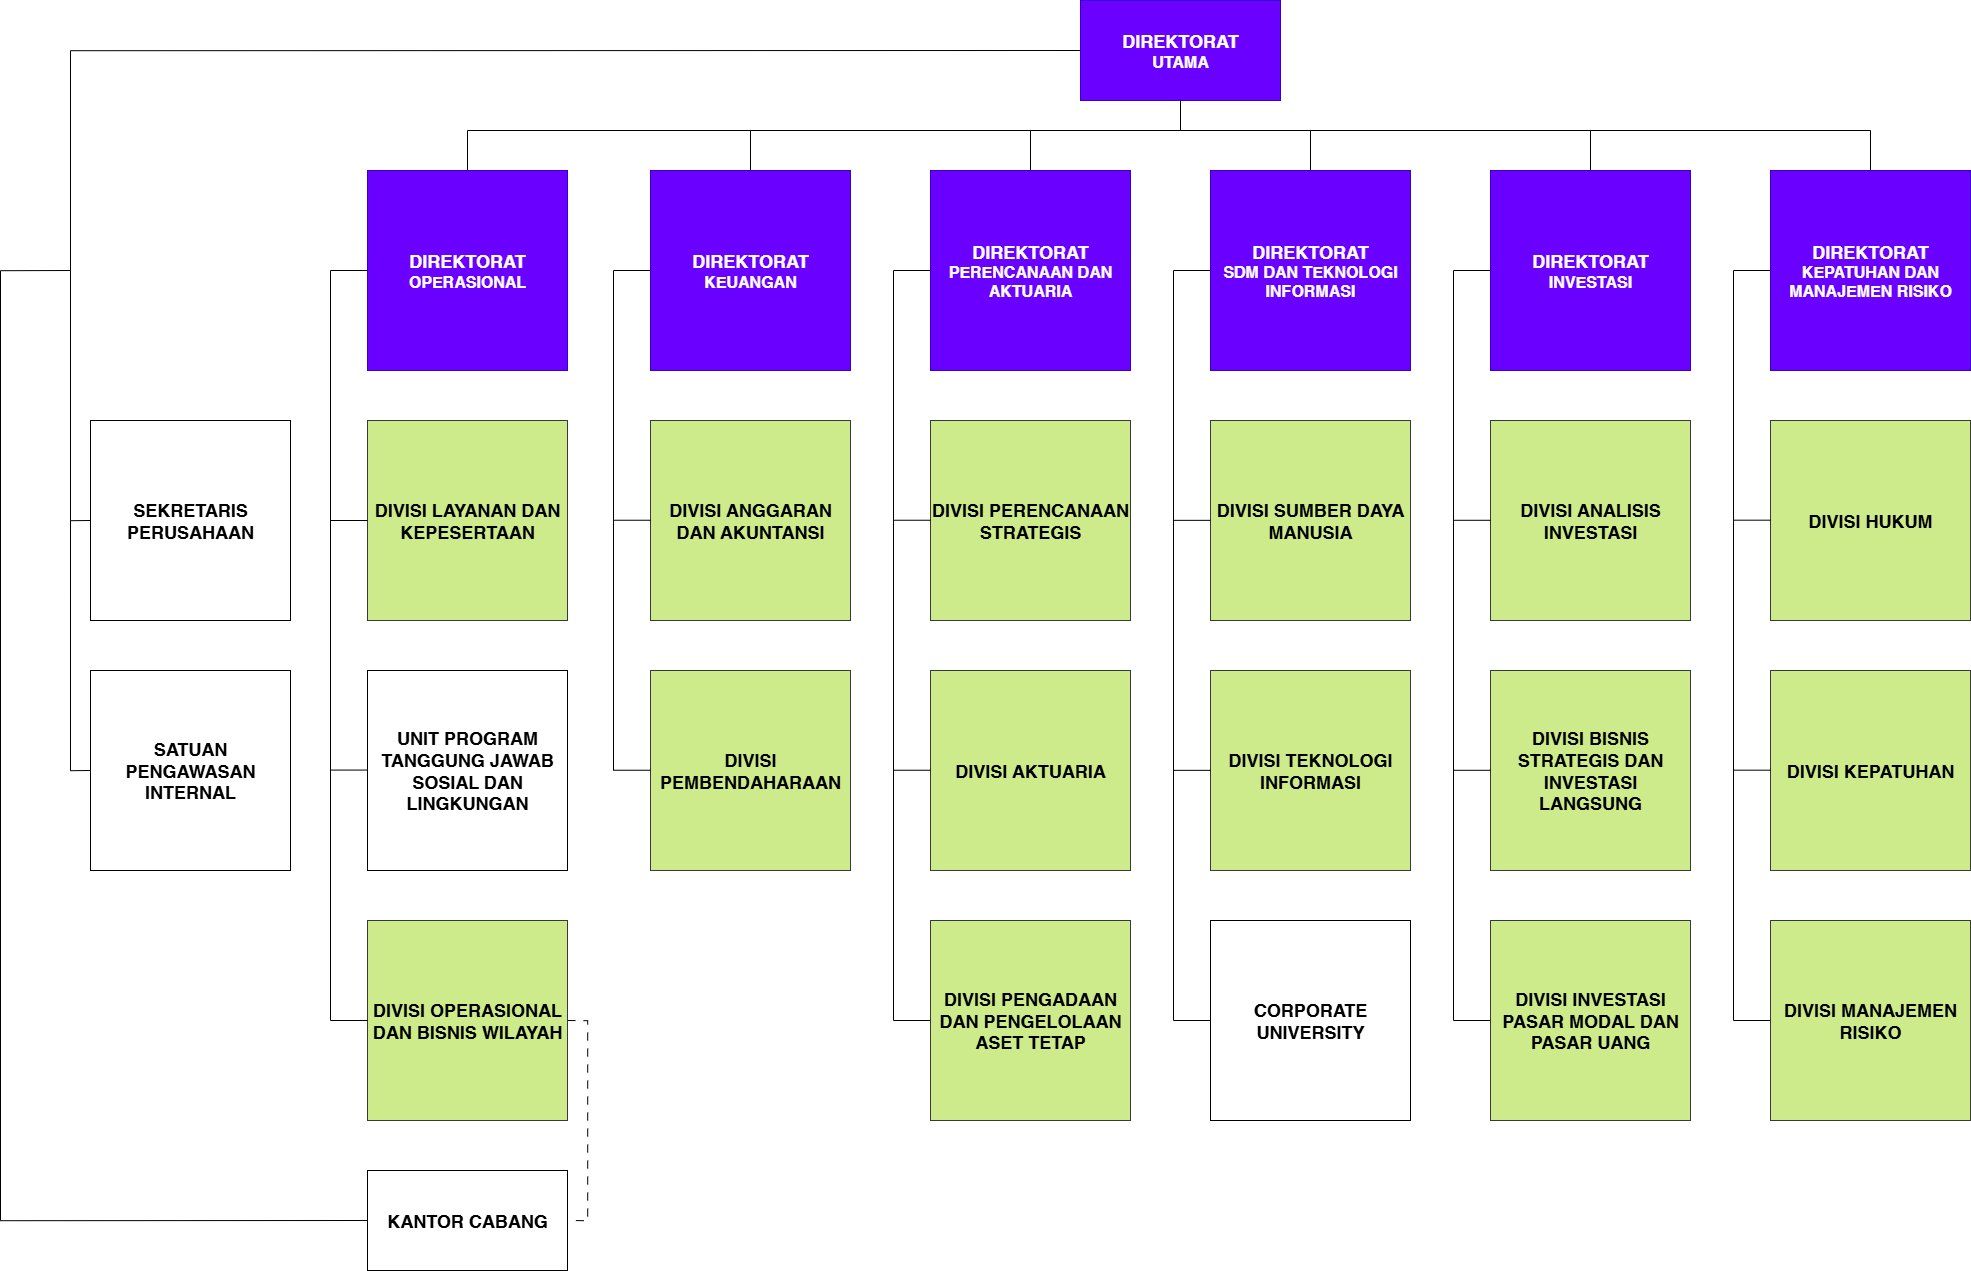
\includegraphics[width=\textwidth,keepaspectratio]{assets/pics/struktur_org.png}
	\caption{Struktur Organisasi PT TASPEN (Persero). Diadaptasi dari Struktur Organisasi, oleh PT TASPEN (Persero), n.d., dari \url{https://taspen.co.id/tentang-taspen/struktur-organisasi} \citep{strukturTaspen}.}
	\label{fig:struktur_org}
\end{figure}
\FloatBarrier

Struktur organisasi PT TASPEN (Persero) dirancang berdasarkan pembagian fungsi strategis yang dipimpin oleh seorang Direktur Utama. Secara garis besar, struktur ini terdiri dari enam direktorat fungsional yang saling terintegrasi. Masing-masing direktorat membawahi divisi-divisi spesifik yang menangani aspek teknis mulai dari pengelolaan keuangan, investasi, hingga dukungan teknologi informasi. Selain itu, terdapat unit kerja yang berperan sebagai pendukung dan pengawasan, serta kantor cabang yang tersebar di seluruh wilayah Indonesia untuk memastikan jangkauan layanan secara nasional.

%-----------------------------------------------------------------------------%
\subsection{Posisi Penempatan Pelaksana Kerja Praktik dalam Struktur Organisasi}
\label{sec:posisiPenempatan}
%-----------------------------------------------------------------------------%
Pelaksana ditempatkan di Divisi Teknologi Informasi (TI) PT TASPEN (Persero)
sebagai Mobile Developer Intern. Divisi TI bertanggung jawab dalam pengembangan
dan pemeliharaan sistem teknologi informasi perusahaan, termasuk aplikasi
internal dan eksternal yang digunakan oleh karyawan maupun peserta TASPEN.

Sebagai Mobile Developer Intern, pelaksana berada di bawah supervisi tim
pengembang aplikasi mobile yang bertugas mengembangkan aplikasi Easy Mobile.
Pelaksana bekerja sama dengan mentor dan anggota tim lainnya dalam menyelesaikan
tugas-tugas pengembangan fitur aplikasi.
